\section{Literature Review}

\subsection{Background}
Practitioners quite often run into an exaggeration of past issues while trying to leverage recent technologies in a rapid pace. In cloud native world the network is unreliable, thus while developing bigger and more dispersed systems, the network needs to be taken into account from the outset of application design (\cite{posta2022Design}). Implementing network resilience like retries, timeouts, circuit breakers, observability and security became challenging for application developer hence a decentralized application networking infrastructure was born as service mesh. Istio is one such open source implementation which has been used for a while now and battle tested by many corporations with their business deliveries. Istio specifies an architecture consisting of a control plane for proxy management and a data plane for network traffic and security management on behalf of an application using application layer proxies (\cite{posta2022Layers}). These application-layer proxies sits as a sidecar within the Kubernetes environment and attached to each service workloads making it a tightly coupled relation with the service deployments. Istio's sidecar proxy injection provides significant advantages over microservice code refactoring for non functional requirements, but do not offer a perfect separation between applications and the Istio data plane (\cite{istioHoward2022}). The Istio community practitioners and contributing companies explored the options of having a less invasive and better ergonomic approaches in service mesh  from last couple of years and Ambient mesh was born. It is now possible to get rid of sidecar architecture in Istio by introducing a shared agent model running per host wise. This gives the operator a lot of cost benefit, flexibility and also provide interoperability with previous generations of service meshes with sidecars. Essentially ambient mesh brings a lot of new excitements in the service mesh space without compromising any purposes that it was invented for.

\subsection{Service Mesh Origins}
During the early days of the Internet, applications used to ship their own TCP/IP stack. This implies that all networking layer code either used to be packaged with the applications or the language specific libraries used to be linked with the application binaries. With the next generation of application development people started shifting towards a shared library model which is still the case with many desktop or embedded applications. Then the creation of the three-tiered application architectural paradigm, which served as the basis for the vast majority of web applications followed by the service-oriented architecture changed the techies to think the way they handled things previously. With this new decoupled service-oriented architecture, additional requirements related to visibility, connection, and security have emerged. Resiliency became more and more important including application components communication over non trusted networks beyond cloud and premises boundaries, and security advancement to a point where sender and recipient can authenticate each other's identities.

\begin{figure}[ht!]
    \centering
    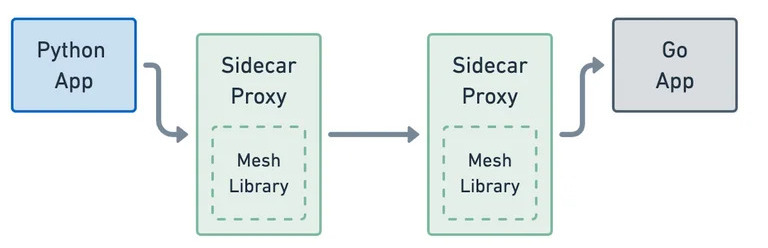
\includegraphics[width=0.7\linewidth]{resources/sidecar-design.jpg}
    \caption{Sidecar proxy design (\cite{isovalentGraf2021})}
    \label{lr:sidecarDesign}
\end{figure}

Implementing all these functionalities out of the application or shared libraries was a big task and making them available as part of the infrastructure for use by all applications was another big challenge. As a solution, sidecar model was introduced which eliminates the need to modify each application separately and supported the polyglot nature of microservice development to best suite the business needs or expertise. The term 'sidecar' was adopted as it attached to the microservices much like a sidecar attached to a motorcycle. This sidecars are now placed with each Kubernetes workload to anticipate network or security movements inside a cluster to form a service mesh delivering speed to the development teams to focus on business logic. Overall, service mesh is a way to connect multiple services to one consistent network and observability layer (\cite{posedioNeumer2021}).

\subsection{Moving from Shared Library Model to Kernel Model - Check}
\label{lr:ebpf}
Historically, the operating system has always been an ideal place to implement observability, security, and networking functionality (\cite{ebpfIODocs}). As operating system implements the central controller unit called kernel, it holds the unique capacity of monitoring and managing the entire system. Over the period of time innovation at kernel level has been lower as its tend to be more complex than functionality outside of it, but with eBPF, that has changed in last few years. What JavaScript did to the browser to change the way today's web application works, eBPF is doing the same at Linux Kernel space. eBPF is a revolutionary technology that runs sand-boxed programs in kernel without modifying the kernel source code or injecting an external kernel module to extend its functionality. Essentially, its a run time in kernel including a JIT compiler to compile byte codes into machine code for execution, making it very optimized and similar level of performance as  native kernel code. eBPF adds the dynamic ability to program kernel by removing back and forth calls between kernel and user space. eBPF works at kernel and user space level by a event driven hook pattern. These events include the entry or exit from any routine in kernel or user space, trace points, and most importantly the arrival of network packets which is crucial for any service mesh (\cite{thenewstackRice2021}). This makes eBPF extremely useful at host level networking observability, security and traffic management.

\begin{figure}[ht!]
    \centering
    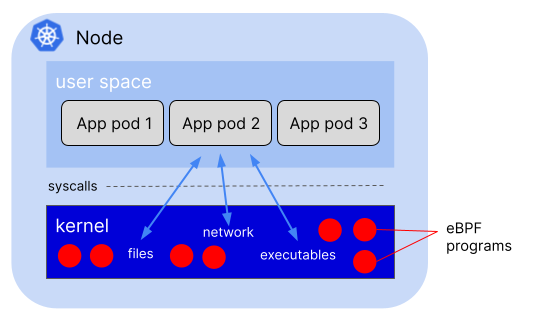
\includegraphics[width=0.7\linewidth]{resources/ebpf-service-mesh.png}
    \caption{eBPF implementation of service mesh (\cite{thenewstackRice2021})}
    \label{lr:ebpfDesign}
 \end{figure}

 As there is only one kernel per Kubernetes nodes, this eBPF technology has become prominent for the service mesh development as this allows to have only one dynamic program for the kernel to serve the service mesh functionalities. This eBPF application program acts as a proxy, but in this case instead of attaching to each pods in Kubernetes cluster, it is attached to the Kubernetes nodes kernel. When attaching proxy to the kernel, a one to one mapping is formed between kernel and proxy eliminating the need of injecting sidecar proxies per pod wise. The evolution from shared library to sidecar and now the kernel model for non-functional requirements in applications development have really gone through a massive change and at each stage the significance was clearly seen by the practitioners.

\subsection{Ambient Mesh Architecture}
With Istio 1.18.0 release in June 2023, the first alpha version of Ambient mesh is launched. This new release gives an option to run Istio installation with ambient parameter to forgo sidecar proxies in favor of a mesh data plane integrated into Kubernetes infrastructure (\cite{istioHoward2022}). To understand Ambient mesh architecture a quick look into Istio sidecar or standard architecture is required. Istio standard has a data plane and a control plane. The data plane is the sidecar proxy which is injected to each Kubernetes pods to monitor, handle and response to events and provide necessary details to and from the service to the mesh network. Control plane remains the controller unit for these data planes and generally its centrally located in the cluster. Ambient mesh divides the data plane into two segments, secure overlay layer or L4 processing layer and L7 processing layer. This layering gives the flexibility to the operator to use the basic potential of a service mesh by deploying L4 processing layer only, reducing the overhead to the entire Kubernetes cluster. The layered approach also helps in migration from no mesh system to secure overlay and to full L7 processing. Next two paragraphs will explore these layers along with the Ambient mesh components which forms the sidecar less architecture.

\subsubsection{L4 Secure Overlay Layer}
Layer 4 of the OSI model represents the transport layer which provides a transparent view of data transfer between end users. Traditionally service mesh incorporates both L4 transport layer and L7 application layer in a single sidecar entity, but in Ambient mesh this is separated and a new zero trust proxy or Ztunnel is introduced. This component is written from ground up using one of the most efficient programming language Rust which naively supports network optimizations and packet filtering. Ztunnel concentrates on a limited number of capabilities, such as mTLS, authentication, L4 authorization and telemetry for Kubernetes workloads without interrupting or processing application level HTTP headers (\cite{istioSun2023}). Ztunnel is deployed as a daemon set on every Kubernetes nodes to process the basic service mesh capabilities. It also forwards the request to the intended app after gathering L4 metrics such as the quantity of request or response bytes. When the target application is running on a different node it ensures that the data is sent to the respective Ztunnel over a secure mTLS connection. The following diagram illustrates how Ztunnel intercepts communication for every pod that is deployed on the same node.

\begin{figure}[ht!]
    \centering
    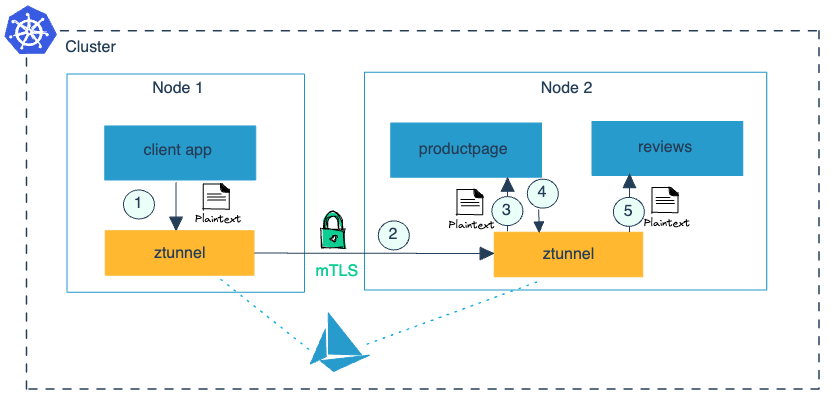
\includegraphics[width=0.7\linewidth]{resources/ambient-routing-l4.png}
    \caption{In cluster routing with Ztunnel in Ambient mesh}
    \label{lr:ztunnelDesign}
 \end{figure}

 \ref{lr:ztunnelDesign} depicts how a client application accept requests from end user to serve a product page along with its reviews. The application runs on a Kubernetes cluster with 2 nodes where the UI, product and review microservice pods are spread across multiple nodes. Each node has its own Ztunnel which internally communicates over mTLS to provide a response back to the end user.

 \subsubsection{L7 Processing Layer}
 Layer 7 works at the highest level of OSI model where application details are available, hence a detailed HTTP level filtering can be done. L7 processing is intensive as it intends to provide connectivity, shape the traffic, apply policies and provide mTLS for microservices running across nodes. This intensive layer analyzes a lot of data and processes a massive scale of network traffic utilizing more CPU and memory resources. To reduce this burden, Ambient mesh introduces a shared component called Waypoint proxy which works at per namespace or per Kubernetes service account level. Waypoint proxies are deployed as a pod and can be placed in any Kubernetes nodes irrespective of where the microservice pods are hosted. The Waypoint proxy forwards the request to the Ztunnel running on the same or different node as the destination microservice, but not before enforcing the L7 rules and gathering L7 metrics (\cite{glooDocs}). By default, mTLS is used to secure traffic between Ztunnel and the Waypoint proxy.

 \begin{figure}[ht!]
    \centering
    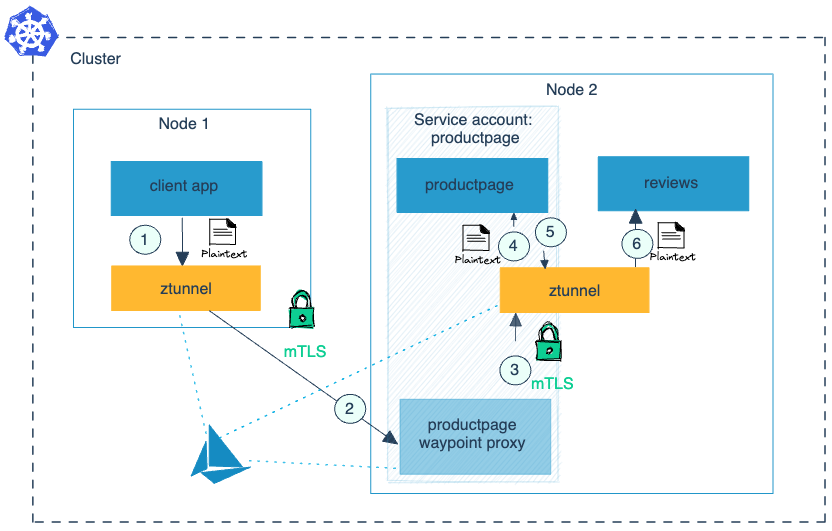
\includegraphics[width=0.7\linewidth]{resources/ambient-routing-l7.png}
    \caption{L7 routing in Ambient mesh}
    \label{lr:waypointDesign}
 \end{figure}

 As shown in the above diagram, the Waypoint proxy is deployed in the product page service account. The request from client application first reaches to the Ztunnel of the client app and then routed to the Waypoint proxy. This is possible as L7 traffic policies are applied to the product page. On receiving the request, Waypoint proxy performs the L7 processing such as collecting metrics and forwards it to the Ztunnel of the corresponding node where the product page microservice pod is running.

 \subsection{Value Proposition of Ambient Mesh}
 A few grey literature describes, using sidecar less model one can reduce the number of proxy instances significantly. One of the empirical study (\cite{thenewstackRice2021}) mentions about using a service mesh built on top of eBPF technology can cut down the proxy counts from 100 to just 3 in a complex Kubernetes cluster used in production. In some other articles, the problem of sidecar proxies are discussed from a real life scenario. \cite{mediumSinghal2021} mentions how they faced an massive increase in memory usage per proxy from 60 - 70MiB to 700MiB - 1.2GiB when they shifted from a small Kubernetes cluster to a larger one. The root cause was identified in the same article and the solution was to restrict the proxy to the required namespaces so that it does not ingest network traffic data for all the services running in the cluster. But even with this limited proxy configuration, per node memory utilization could reach up to a significant number when the service replica increases due to auto scaling. Kernel mode service mesh not only reduces this memory footprint, but it can also reduce the complexity of having less YAML, application pod restart when rolling out the service mesh in a live cluster. Though the focal point of the kernel mode service meshes like Ambient mesh remains at the performance side but the reduced operational complexities can not be ignored. One of the most significant benefits of switching to Ambient mesh is two layers of network traffic filtering. Ambient mesh allows incremental adoption by applying secure overlay processing by default and high level HTTP based L7 processing on demand. This two layer architecture enables organizations to pay for what is needed and scale the service mesh data plane independently from the Kubernetes workload reducing the infrastructure cost (\cite{infoqSunCampbell2023}).

 \subsection{Summary}
 Ambient mesh offers advantages over sidecar based deployment model due to its noninvasive and leaner design. Adoption of the ambient mesh directly reduces infrastructure costs and improves performance because it involves fewer components - Ztunnel proxies per node and the optional Waypoint proxy. The design also allows for separating L4 and L7 processing, giving the operator a granularity on control and choice. Though the introduction of Ambient mesh does not mean the end of sidecar model in service mesh, there is a lot of potential which Ambient mesh brings today. There are use cases when service meshes with sidecar may remain useful such as in regulatory environments as keeping proxies in the same pod guarantees to be coupled with microservice at the same geographic location which is easy to justify during an audit. Despite of few exceptional cases, ambient mesh will remain as one of the most exciting technology in service mesh field which leverages the Linux kernel eBPF technology. As there is no academic research paper available at present, an immense opportunity is opened to explore Ambient mesh, what it offers and how it is different from standard sidecar mode of Istio.